% This file can be used to compile the adventure into a stand alone PDF without the sourcebook
\documentclass{book}


\usepackage{../../static/templates/fate_latex_template/fate_solarpunk}
\usepackage{montserrat}
\usepackage{ebgaramond}
\usepackage{hyperref}

%%%%%% Fixing overful hboxes
%% https://tex.stackexchange.com/questions/35/what-does-overfull-hbox-mean-why-is-there-a-black-mark-at-the-end-of-a-line
\usepackage{hyphenat}
%% \hyp{} can mark where words can break
%% Make it simpler:
%% https://tex.stackexchange.com/questions/488008/how-to-create-an-alternative-to-shortcut-or-hyp
\usepackage[german]{babel}

% Create title and background image
% https://tex.stackexchange.com/questions/136900/insert-a-full-page-image
% https://www.ctan.org/pkg/background
\usepackage[pages=some]{background}
\backgroundsetup{
scale=1,
angle=0,
opacity=1,
firstpage=true,
contents={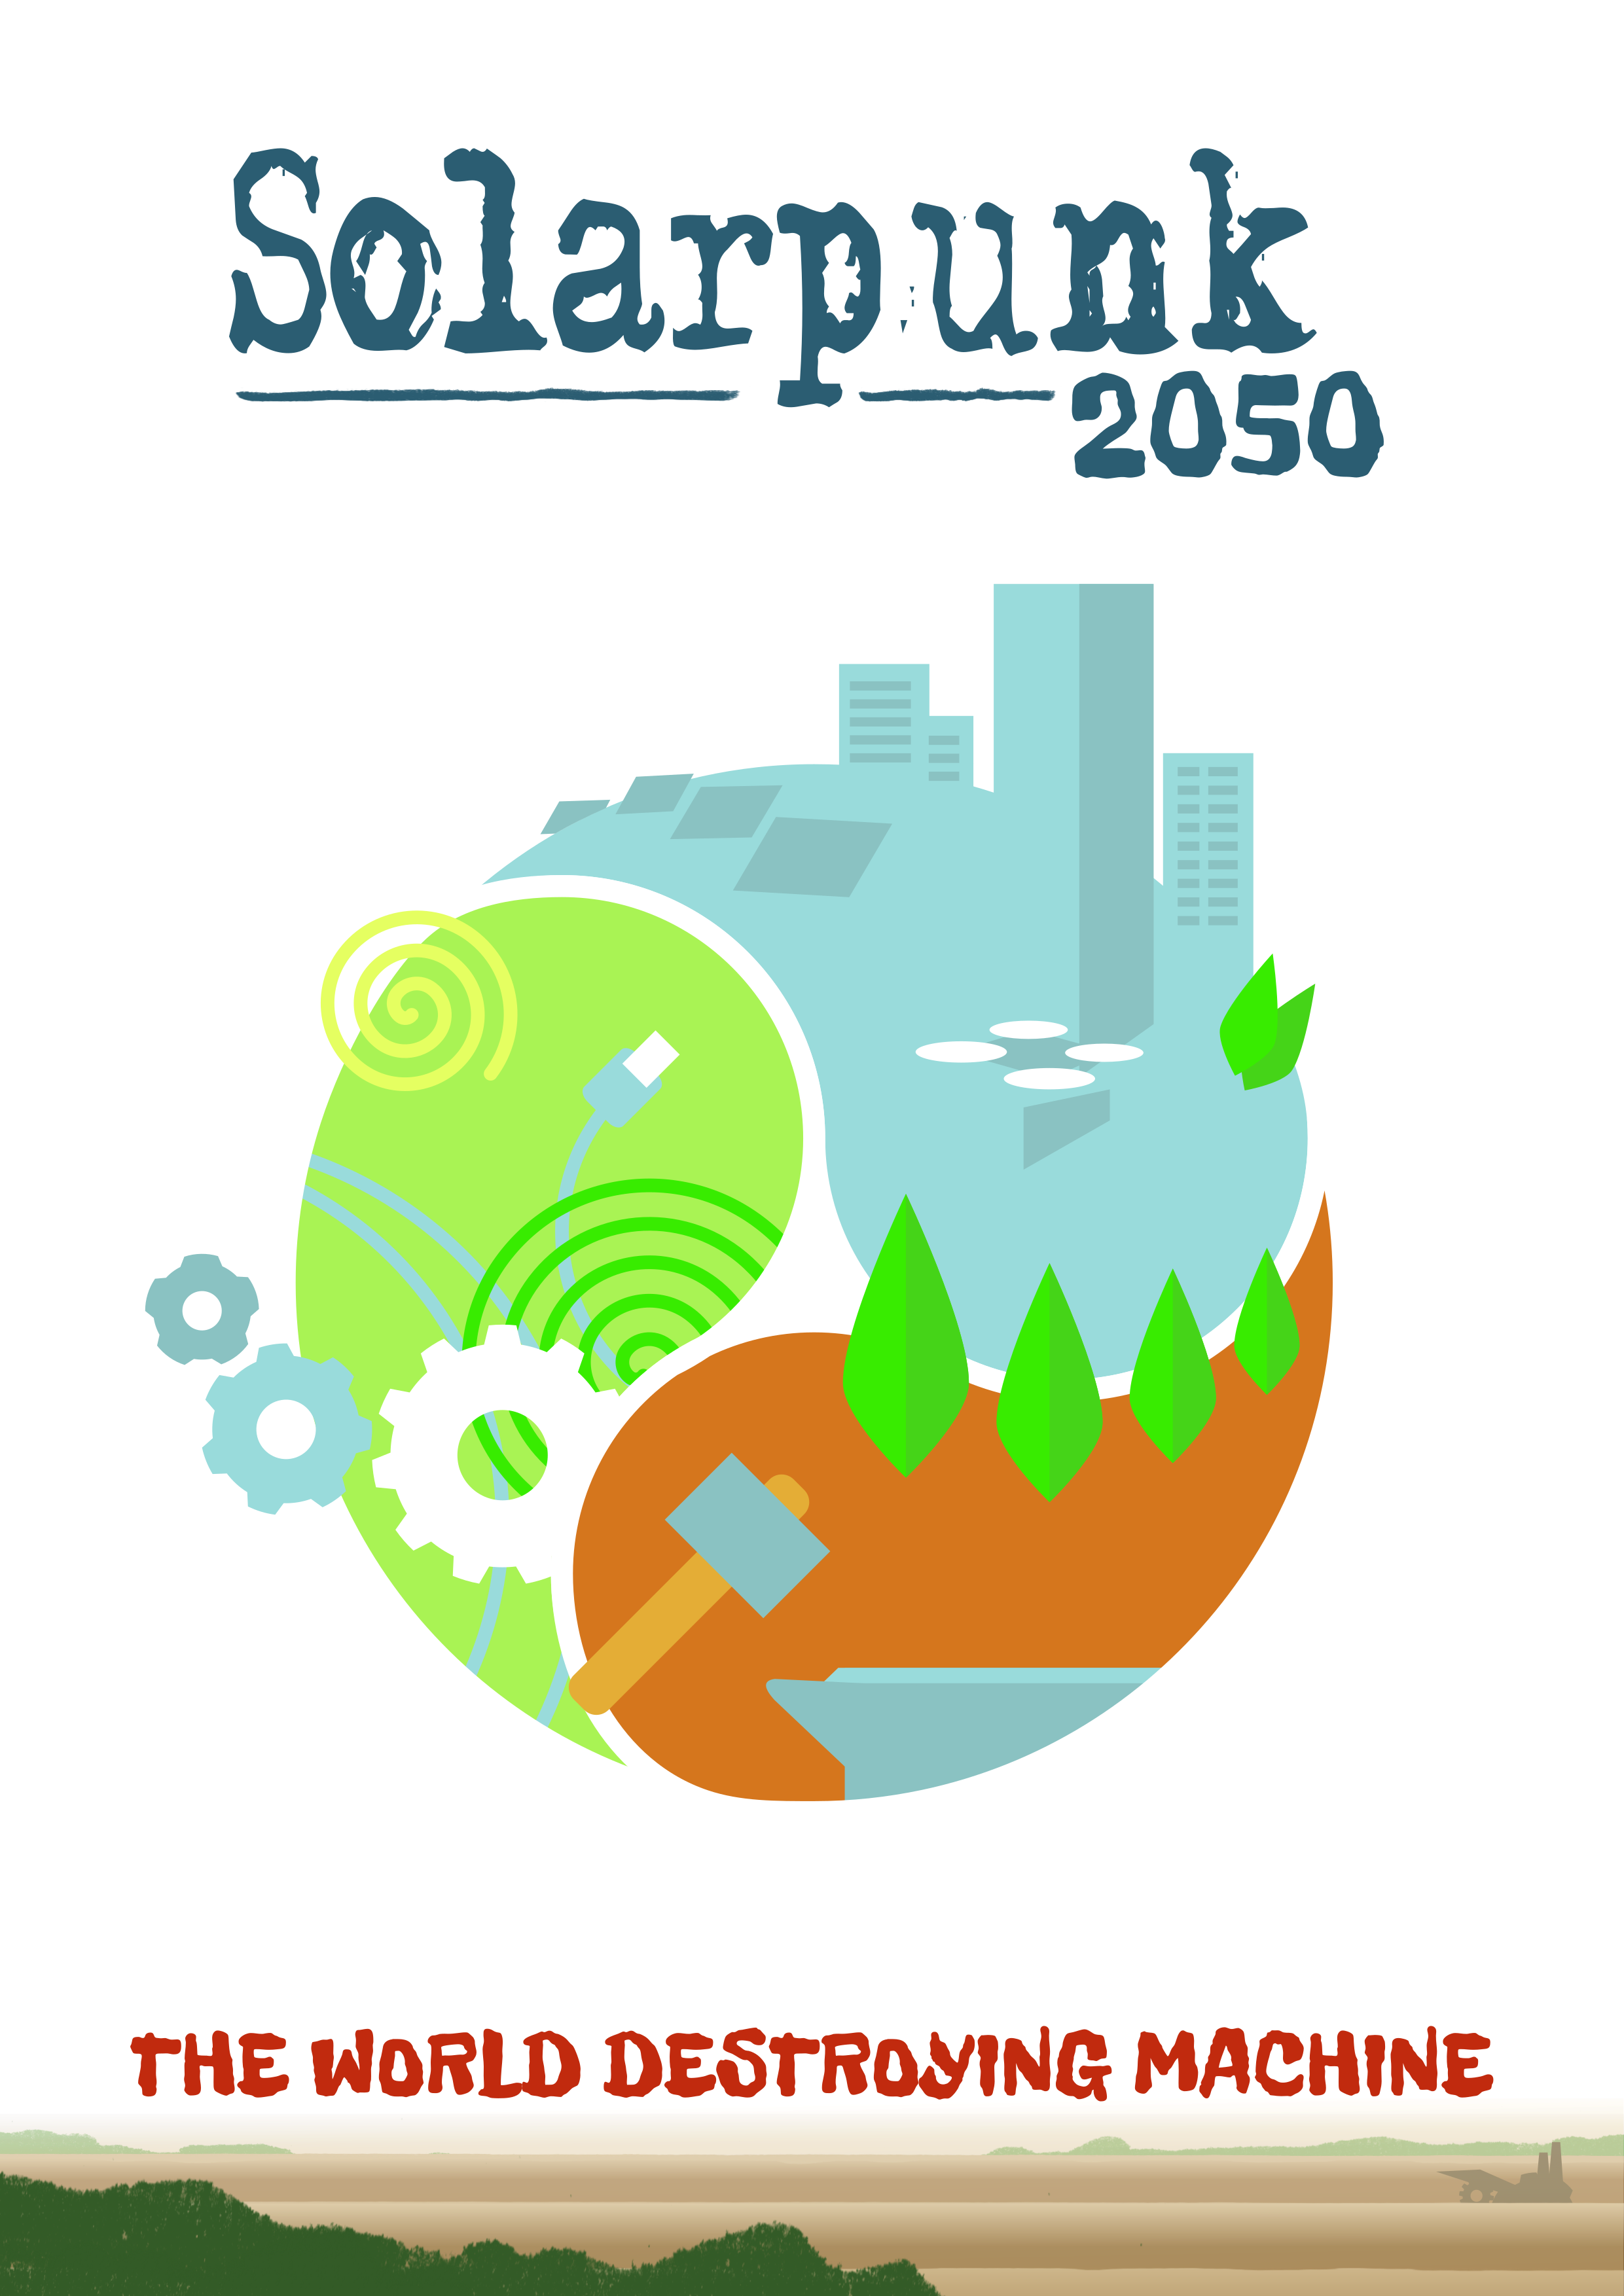
\includegraphics[width=\paperwidth,height=\paperheight]{../sourcebook/static/Solarpunk-Machine.png}}
}

\useshorthands{~}
\defineshorthand{~-}{\hyp{}}
%% ~- can mark this break now



%... other code

% \section{Hello World}
% \label{sec:hello}



% For creating example text
% \usepackage{lipsum}

\title{Fate Solarpunk 2050 - Kollektion: Der Flohmarkt}
\author{Thorsten Sick}

\pagenumbering{arabic}
\begin{document}

%
% Book front page
%
\mbox{}
\thispagestyle{empty}
\BgThispage


%% Hyphenation database:
\hyphenation{meal-worm Mc-Gyver fa-mous be-cause}
%%%%%

%% Ziele: Story hooks
%% Mehr Drama als eine Telenovella
%% Man muss zig Abenteuer aus der Konstellation ziehen können
%% Die Meisten Charaktere sind ü 60 und haben viel erlebt. Das aufzählen.

\chapter{Der Lost Flohmarkt}

Es gibt mehrere Lost Flohmärkte. Dieser hier ist ein mobiler, durch die Lande ziehender Flohmarkt und Treffpunkt verschiedener Lost Gruppen. Doch auch einige Norms und Pioneers werden von diesem angezogen und of verwirrt zurück gelassen.

Für die Lost ist die Funk Nachricht, dass bald ein Flohmarkt in ihrer Nähe stattfinden wird ein wichtiges Ereignis. Doch diesen zu organisieren bedarf einiges an Aufwand und spezieller Menschen.

Am wertvollsten sind die Artefakte aus der alten Welt, die die Lost bei Expeditionen geborgen haben. Die Artefakte der Lemminge. Insbesondere die Lost sind auf alte Technologie angewiesen, um ihre Fahrzeuge und Gebäude zu reparieren.

Lost handeln übrigens im Tauschhandel, Norms bezahlen mit digitalem Geld und bei Pioneers finden viele Transaktionen eher über Ruf und Ruhm der Personen statt. Auf einem Lost Flohmarkt sind also gerade für nicht-Lost Kulturschocks und chaotische Ketten an Tauschhandel vorprogrammiert.

\chapter{Die Aufgabe}

Das Team des Flohmarkts reist durch die Lande, kündigt einen Flohmarkt an, organisiert einen Platz und beginnt diesen herzurichten für um die 500 Personen. Viele der dazukommenden Lost werden zwar selbst beitragen (eigene Essens Stände, Werkstätten).
Doch das Team stellt die basis Infrastruktur zur Verfügung und versucht verfeindete Gruppen zusammen zu bringen. Denn das ist der sinn des Flohmarkts (neben Tauschhandel, Wissensaustausch, Unterhaltung).

\section{Die Probleme}

Beim Aufbau des Lost Flohmarktes kommt es natürlich zu einer Reihe von Problemen. Diese müssen von den NSCs, den Protagonisten und evtl. den neu hinzugekommenen Gruppen gelöst werden. Sollte die Situation mit externen Charakteren als Protagonisten gespielt werden, wäre es eine coole Herausforderung, die Flohmarkt-NSCs die großen Herausforderungen stemmen zu lassen, und denPc Protagonisten die Rolle des Steine-aus-dem-Weg räumens und als Katalysator zukommen zu lassen.

\begin{itemize}
\item Eine Gruppe kommt zu spät
\item Eine Gruppe kommt zu früh
\item Das Feld auf dem der Flohmarkt stattfinden soll ist nach Starkregen ein See. Mit Brennesseln und Gestrüpp. Der muss zuerst mit schwerem Gerät trocken gelegt werden.
\item Beim trockenlegen wird eine verschüttete Lemmings Ruine gefunden. Schätze daraus wollen von den Jones-es geborgen werden. Das kann zu einem Dungeon Crawl führen.
\end{itemize}

\chapter{Die Personen}

\section{Heavy machines: Wendy}

Chef Logistikerin, Heavy machines und Truckerin: Wendy früher Wilhelm. Ihre Ehe hat sich vor der Katastrophe zerrüttet. Sie wusste auch nicht warum. Hat erst spät festgestellt, dass sie Trans ist. Hat ein Foto aus der Alten Zeit hinter der Sonnenblende. er zusammen mit Doris. Auch mit dem Truck durch Europa unterwegs. Dass Wendy mal Wilhelm war, wissen die Lost nicht.

\section{Norm Dokumentatorin Doris}
Sie ist auf Abenteuer Trip (ohne Sanitäre Einrichtung und ohne Kunstfleisch/Drohnen/Vernetzung): War früher mit Wilhelm verheiratet. Trägt immer noch den Ring in ihrer Tasche, weiss nicht, dass es Wendy ist. Kommen sie wieder zusammen ?

\section{Pioneer Tochter "Flash"}
Die Tochter von Doris und Wilhelm. Auch so 35 Jahre alt. Aber sehr aktiv und unstet. Ist mit ihrer Mutter leicht zerstritten (wegen ihr kein Kontakt zum Vater, und sie ist eine langweilige Norm). Weiss aber, dass der Vater Wendy heisst und bei den Lost ist, Hat keine Ahnung, wie sie sich vorstellen soll. Für sie ist eine originelle Geschlechts identität absolut üblich in ihrem Umfeld.

\section{Tier Experte}

Organisiert die Unterbringung der Tiere (von Hasen bis zu Rindern). Sorgt für die Gesundheit der verkauften Tiere und hilft bei der Futterversorgung. Ist aber eigentlich Tiertrainer für Raubvögel. Diese Reissen aber manchmal Hasen - auch solche in den Freigehegen der Farmer.

\section{Küche und Militärtaktik}
"Zwischen dem Führen einer Küche und einer Schlacht Organisation gibt es kaum Unterschiede". Führen kleiner Einheiten. Zur Lager Verteidigung oder beim Kochen für einen Flohmarkt. https://de.wikipedia.org/wiki/K%C3%BCchenbrigade
Feldküche und Feld Taktik

\section{Funk und Kommunikation}
Kennt jeden, kann viele Sprachen. Will Happy Hippo komplett bekommen: Fragt bei seinen Funk Kontakten rum und kann evtl. eine Bergungstrupp losschicken wollen.

\section{Gaia Priester}
Gaia Priester haben sich der lebendigen Gaia verschrieben. Der Einheit der Öko/Techno und Soziosphäre.Sie versuchen besonders, andere Leute zu animieren,  Brücken zu bauen. Brücken zwischen verfeindeten Gruppen z.B. und dabei gemeinsam Projekte umzusetzen.


\chapter{Andere Gruppen}

Lost Flohmärkte wollen gezielt mehrere Lost Gruppen zusammen bringen. Doch oft findet man leicht verwirrte Pioneers und Norms.

\section{Jones-es}

So nennt sich eine Gruppe, die in den Ruinen der Lemmingenach Technologie, Büchern und anderen wertvollen oder interessante Dingen sucht. Sie bieten ihre letzten Funde an. Dafür benötigen sie Medikamente und Reperaturen.

\section{Farmer}

Suchen Tiere zur Zucht und Pflanzensamen. Sind bereit mit Naturalien zu zahlen. Deren Tiere können ein Mist-Entsorgungs Problem verursachen und massiven Gestank, wenn man das nicht im Vorfeld einplant.

\section{Handwerker}

Bieten Reperaturen, benötigen aber Rohstoffe.


* Ausgrabungs-Team, die immer was zu verkaufen haben
* Hunderte Lost aus andere Gruppen, die kochen, reparieren, verkaufen, kaufen, vorlesen, musizieren, suchen und einen Jahrmarkt betreiben mit aller Art von Buden



\end{document}